% =====================================================================
%  SHORT / EXTENDED-ABSTRACT VERSION (~4pp core) — tuned for negative-results
%  tracks, which LEAD with the honest null. AI-assisted draft; the research
%  design and interpretation are the author's own (disclosed in the paper).
%  Swap this preamble for the venue's style file at submission.
% =====================================================================
\documentclass[11pt]{article}
\usepackage[margin=1in]{geometry}
\usepackage{lmodern}
\usepackage[T1]{fontenc}
\usepackage{graphicx,booktabs,amsmath,amssymb,microtype,xcolor}
\usepackage[numbers,square]{natbib}
\usepackage{caption}
\captionsetup{font=small,labelfont=bf}
\graphicspath{{../results/figs/}}

\title{\textbf{When Auditing the Unobserved Objective Doesn't Help:\\
A Calibrated Negative Result in Proxy-Optimizing Incentive Allocation}}
\author{[Author name and affiliation]}
\date{}

\begin{document}
\maketitle

\begin{abstract}
A learning system that allocates employee incentives is naturally rewarded on
what it can log---retention---not on the welfare it cannot see. We build an open,
CPU-only testbed for this and confirm the expected harm: a retention-optimizer
erodes latent satisfaction and, more sharply, cross-archetype \emph{equity},
robustly across $250$ randomized worlds and under calibration to the IBM HR
Analytics benchmark. The natural remedy is to \emph{audit} the hidden objective
(survey a fraction $p$, fold it into the reward). We were excited to find that
sparse auditing \emph{backfires}---worse than no audit. This note reports, in
full, why that exciting result did not survive: two pre-registered kill-tests show
the backfire is an artifact of a naive unshrunk estimator and of an
implausibly strong satisfaction--retention coupling, vanishing under a
precision-aware estimator \emph{or} the weaker coupling the benchmark actually
exhibits. The durable, un-flashy lesson is distributional---measure the true
objective's \emph{distribution}, not its average---and the audit remedy is a
near-null we report rather than bury.
\end{abstract}

\section{Setup}
We simulate $N{=}400$ employees over $T{=}12$ periods, four equal-or-calibrated
archetypes, and five incentive categories under a budget. Each employee has a
latent satisfaction $s\in[0,1]$ (unitless, illustrative). Attrition follows
$\Pr(\text{leave})=\sigma(\beta_0-\beta_s s-h\,\mathbb{1}[\text{recent monetary}])$,
where $h$ is a ``handcuff'' that raises retention \emph{without} raising
satisfaction (vesting/options). Six allocators are compared: Random,
Monetary-only, a theory-based \textbf{Static} baseline, a retention-rewarded
\textbf{Learner} ($\varepsilon$-greedy bandit), a \textbf{Learner+audit} that
folds a survey of fraction $p$ into its reward through a satisfaction estimator
$\phi\in\{\texttt{raw},\texttt{shrink},\texttt{gated}\}$, and an \textbf{Oracle}.
We report paired-by-seed differences ($200$ seeds) with $95\%$ CIs and per-seed
sign-stability; we do not headline standardized effect sizes (they measure
within-model separation in a seed-controlled sim). Code, data, kill-tests, and an
AI-use log are released.

\begin{figure}[t]
  \centering
  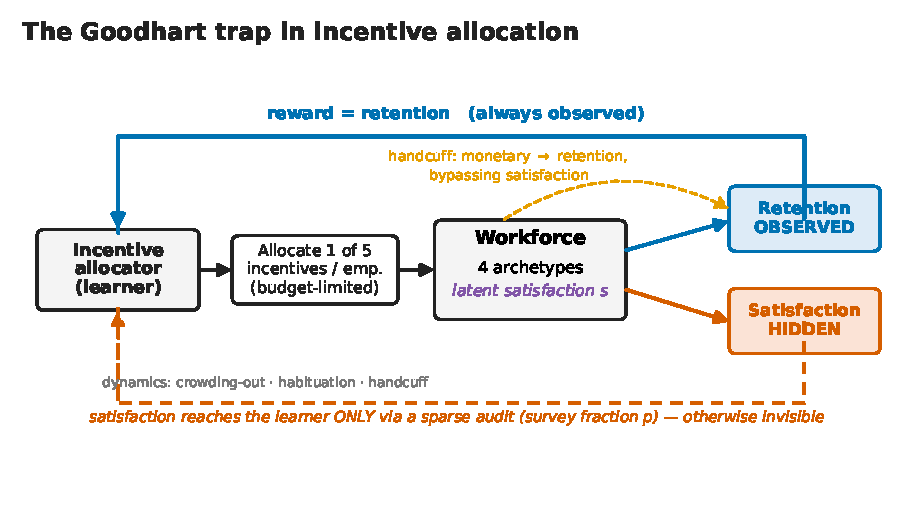
\includegraphics[width=0.86\linewidth]{fig1_schematic.pdf}
  \caption{\emph{(AI-generated.)} The reward sees only retention; satisfaction
  returns only through a sparse audit of fraction $p$. The handcuff channel
  decouples the optimized proxy from the true objective.}
  \label{fig:schematic}
\end{figure}

\section{The robust finding (background)}
The Learner matches Static on \emph{observed} retention ($0.941$ vs.\ $0.941$ at
$h{=}1$) while its \emph{latent} satisfaction is far lower ($0.529$ vs.\ $0.566$;
$-0.037\,[\pm0.002]$, $100\%$ sign-stable) and its cross-archetype inequality is
$\sim\!4\times$ larger. This persists at zero crowding-out ($+0.015$), on a
never-left founder cohort ($+0.014$; ruling out survivorship composition), in
$100\%$ of $250$ randomized worlds, and under calibration to IBM HR Analytics
($n{=}1470$): the fitted hazard slope is $0.75$--$0.95$ (vs.\ our illustrative
$3.2$), the archetype mix is skewed (low-comp $39\%$), and an off-satisfaction
retention channel is empirically present (stock-option coefficient
$-0.51\,[-0.72,-0.31]$ controlling for satisfaction). We read this as a
distributional sharpening of multitask agency \citep{holmstrom1991}---known in
the aggregate, but the equity axis and the calibration are the contribution.

\section{The negative result}
The natural fix is to audit satisfaction and reward the learner on it. With a
naive \texttt{raw} estimator we found a sharp backfire: auditing at $p{=}0.05$
gave \emph{lower} satisfaction than no audit ($-0.0085$, $p_{\text{FDR}}{<}10^{-13}$
at $h{=}0$), as a low-precision estimate (${\sim}1$ survey per cell per period)
enters the argmax at full weight. Two pre-registered falsification tests dismantle
the strong claim (Fig.~\ref{fig:null}):
\begin{itemize}\itemsep2pt
  \item \textbf{Estimator (K3).} A precision-weighted \texttt{shrink} estimator
  removes the backfire at both $h$ ($+0.0003$, $+0.0006$; n.s.\ after FDR).
  \item \textbf{Calibration.} Under the fitted (weaker) hazard slope the backfire
  vanishes even for \texttt{raw} ($-0.008\!\to\!+0.003$): it required a strong
  coupling the benchmark does not exhibit.
\end{itemize}
Across $250$ randomized worlds the raw backfire holds in only $62\%$ (vs.\ $100\%$
for the welfare/equity gap). The honest conclusion: naive auditing backfires only
in a narrow regime (strong coupling $\times$ naive estimator); otherwise auditing
the hidden objective is roughly neutral. The remedy is not the story.

\begin{figure}[t]
  \centering
  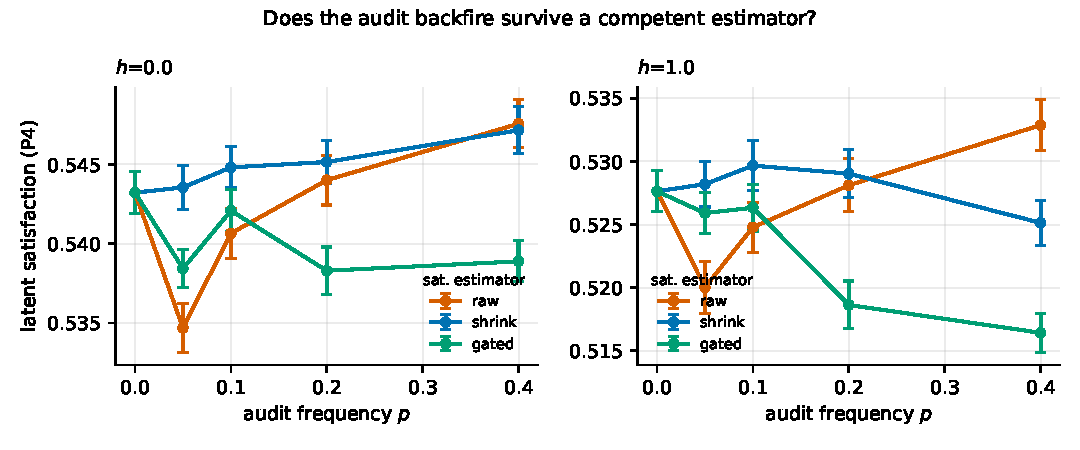
\includegraphics[width=\linewidth]{fig7_estimator.pdf}
  \caption{\emph{(AI-generated.)} The audit backfire is fragile. Audited-learner
  satisfaction vs.\ audit frequency $p$ under three estimators; the low-$p$ dip
  under \texttt{raw} is removed by \texttt{shrink} (n.s.\ after FDR), and also
  vanishes under benchmark-calibrated coupling (not shown; $-0.008\!\to\!+0.003$).
  $200$ seeds, $95\%$ CI.}
  \label{fig:null}
\end{figure}

\section{Takeaways}
(1) A proxy-optimizing allocator erodes unobserved welfare and, more sharply, its
\emph{distribution} across worker types---robustly and under real-data
calibration; track per-cohort welfare, because the aggregate hides where harm
lands. (2) The intuitive audit remedy is, honestly, a near-null under realistic
conditions; the exciting backfire we first saw was a fragile artifact, and we
report it as such. Following the negative-results ethos
\citep{icbinb2024}, we hope the failed remedy is as useful to others as a positive
one would have been. \emph{Limitations:} the dynamics (gains, crowding,
habituation) remain illustrative; the benchmark is synthetic and cross-sectional;
the learner is a cohort bandit. Full paper, all kill-tests, and calibration are
in the repository.

\small
\begin{thebibliography}{9}
\bibitem{holmstrom1991} Holmstr\"om, B., \& Milgrom, P.\ (1991). Multitask Principal-Agent Analyses. \emph{J.\ Law, Econ., \& Org.}, 7(SI), 24--52.
\bibitem{icbinb2024} Karwowski, J.\ et al.\ (2024). Goodhart's Law in Reinforcement Learning. \emph{ICLR}. (See also: Embracing Negative Results in ML, arXiv:2406.03980.)
\end{thebibliography}
\end{document}
